To evaluate the performance of the proposed pipeline, extensive experiments were executed on the \kuka platform of Fig. \ref{fig:new_setup}, to accurately represent the motivating complications that arise in real-world setups. The experiments are designed to showcase the hardness of tight packing as well as the benefits of adding robust environment-aware manipulation primitives that aid in increasing success rate and accuracy. 


\rahul{

\subsection{Real-world Packing Trials}
To evaluate the performance of the primitives over different noise levels and to study the sensitivity of the primitives with respect to the underlying parameters, extensive experiments were executed on a physics-based simulator. The output of {\it real-world experiments} and {\it simulation experiments} are evaluated over two distinct metrics. The {\it volumetric error} measures the percentage of unoccupied volume within the ideal target placement volume. This is measured by computing an occupancy grid based on the sensing data acquired after the objects have been moved to the target bin. Given the partial observation, an approximation of the volume is computed by projecting the sensed points down to the bottom surface of the bin and marking all voxels along the projection as occupied. The second metric is {\it pose recall}. A pose is assigned to each of the object placements by manually aligning a 3D CAD model of the object to the observed point cloud data. This pose is then compared to the closest target pose to compute an average distance (ADI) error \cite{hinterstoisser2012model} that is often used in the pose estimation literature. Given two poses, the ADI metric measures the average distance between corresponding points on the object model placed at the two poses. A pose is considered correct if the ADI error is less than a distance threshold. Pose recall curves indicate the number of successful object placements that are within different threshold margins.


}


\begin{figure*}[ht]
\centering
  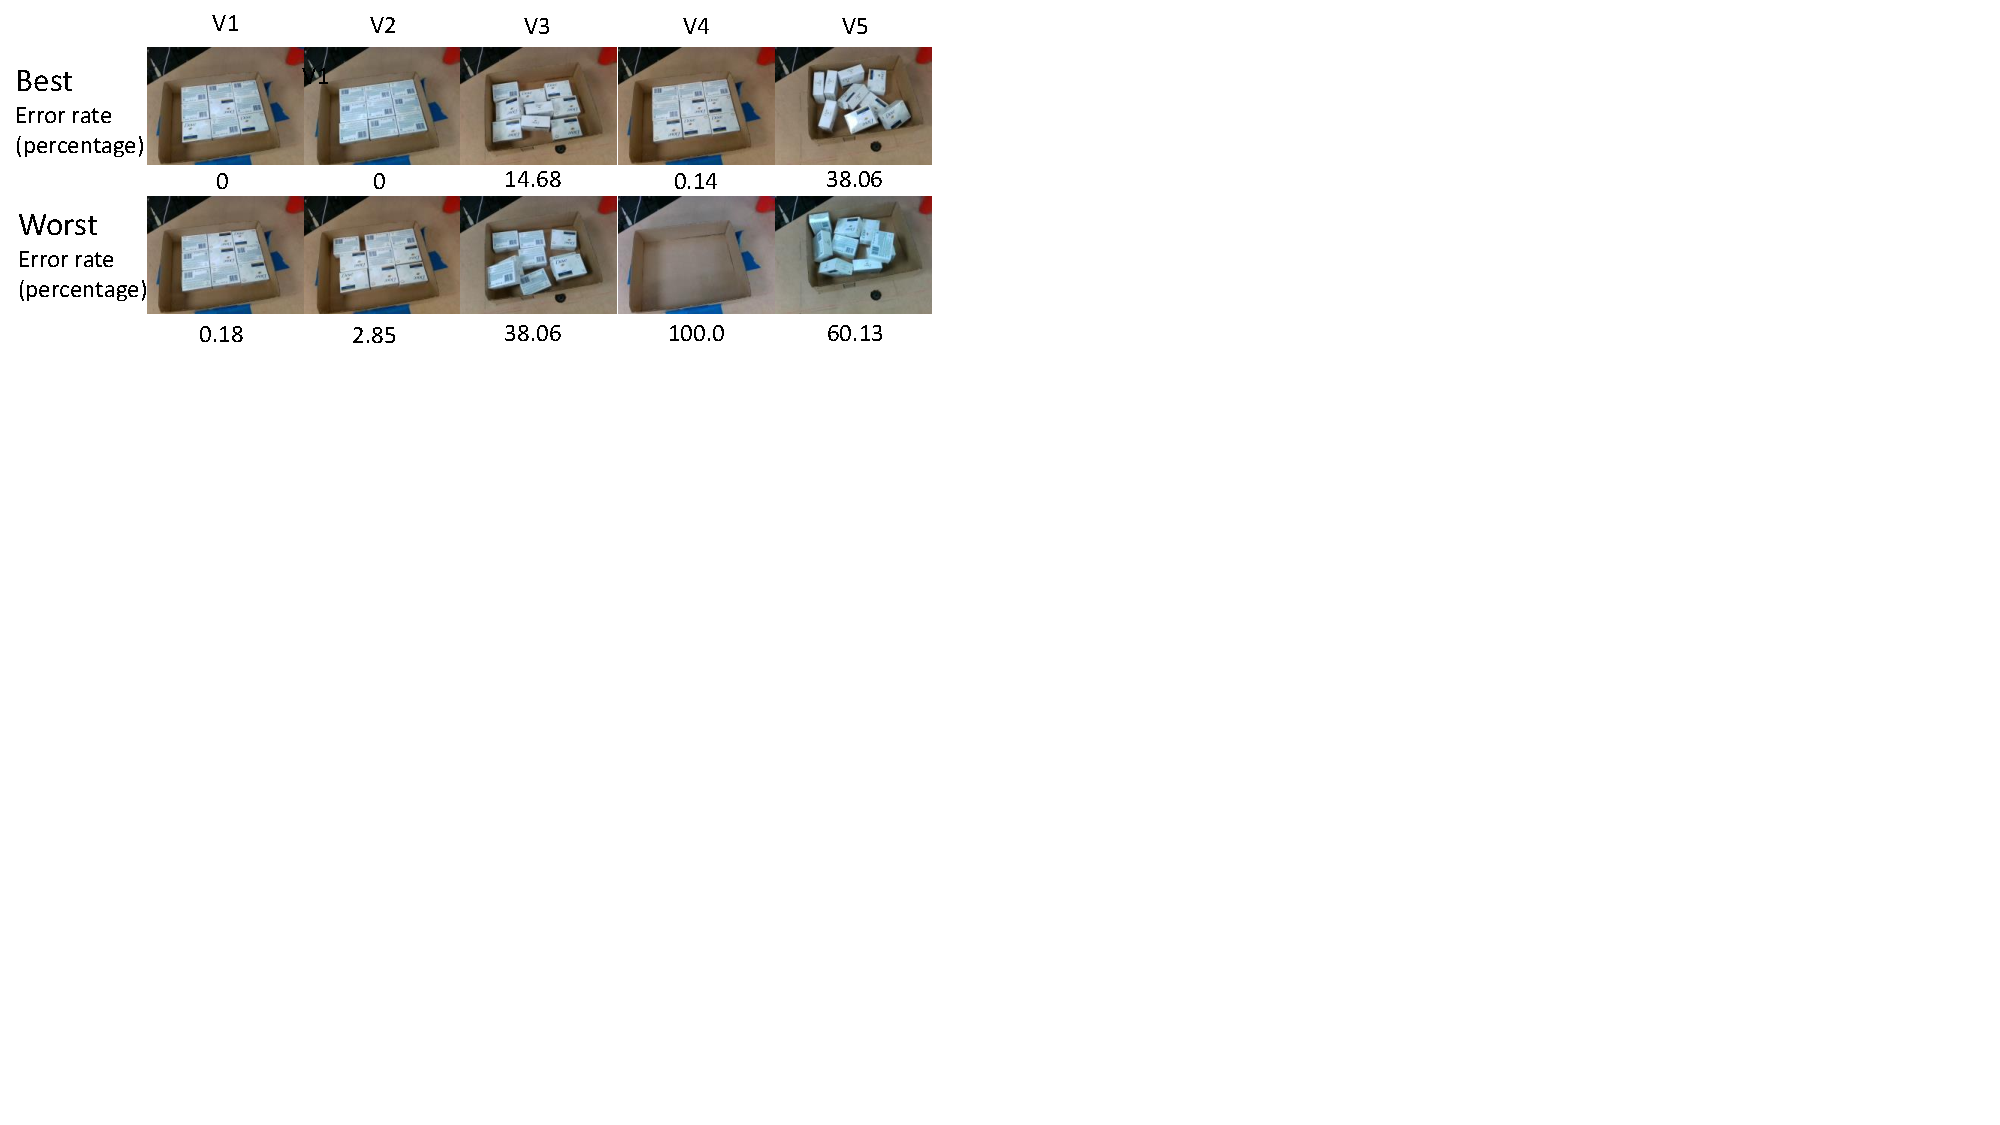
\includegraphics[width=1\textwidth]{Figures/final_packing.pdf}
  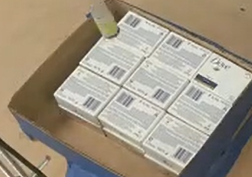
\includegraphics[height=1.1in]{Figures/two_layer.PNG}
  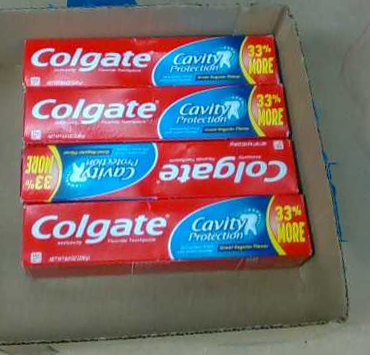
\includegraphics[height=1.1in]{Figures/toothpaste.png}
  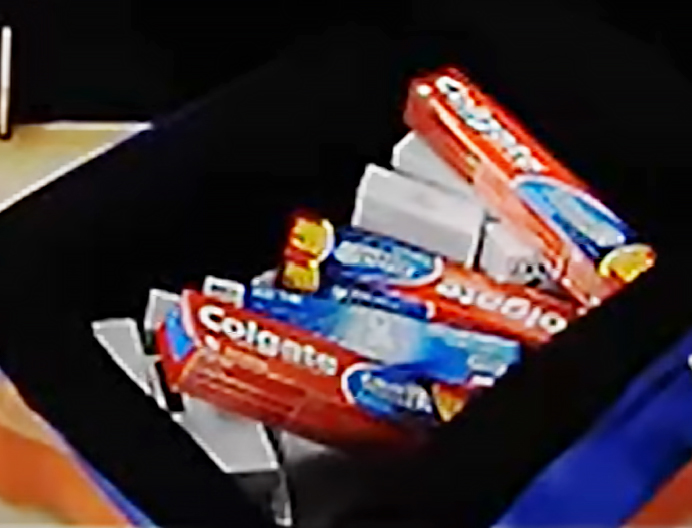
\includegraphics[height=1.1in]{Figures/two_object}
  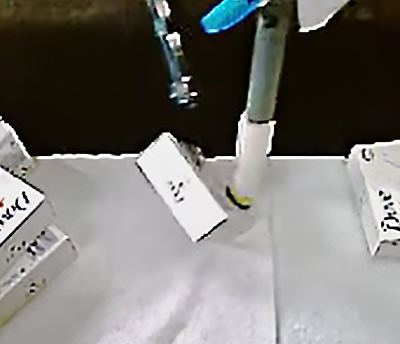
\includegraphics[height=1.1in]{Figures/flat_topple}
  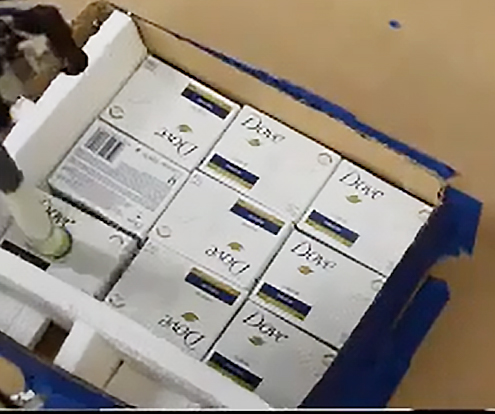
\includegraphics[height=1.1in]{Figures/tight_packing}
\vspace{-0.1in}
\caption{The final set of object poses in the target poses at the end of every experiment. Different column represents different versions. The \textit{top row} is the best case, and the \textit{middle row} is the worst case. (\textit{Bottom row: }) Demonstrative real-world trials performed with the same pipeline for (\textit{left to right}) multi-layer packing, different objects, heterogeneous piles, narrow-face toppling, and no-clearance packing.
}
% \vspace{-0.2in}
\label{fig:final_bin_configs}
\end{figure*}

\begin{figure*}[h]
\centering
% 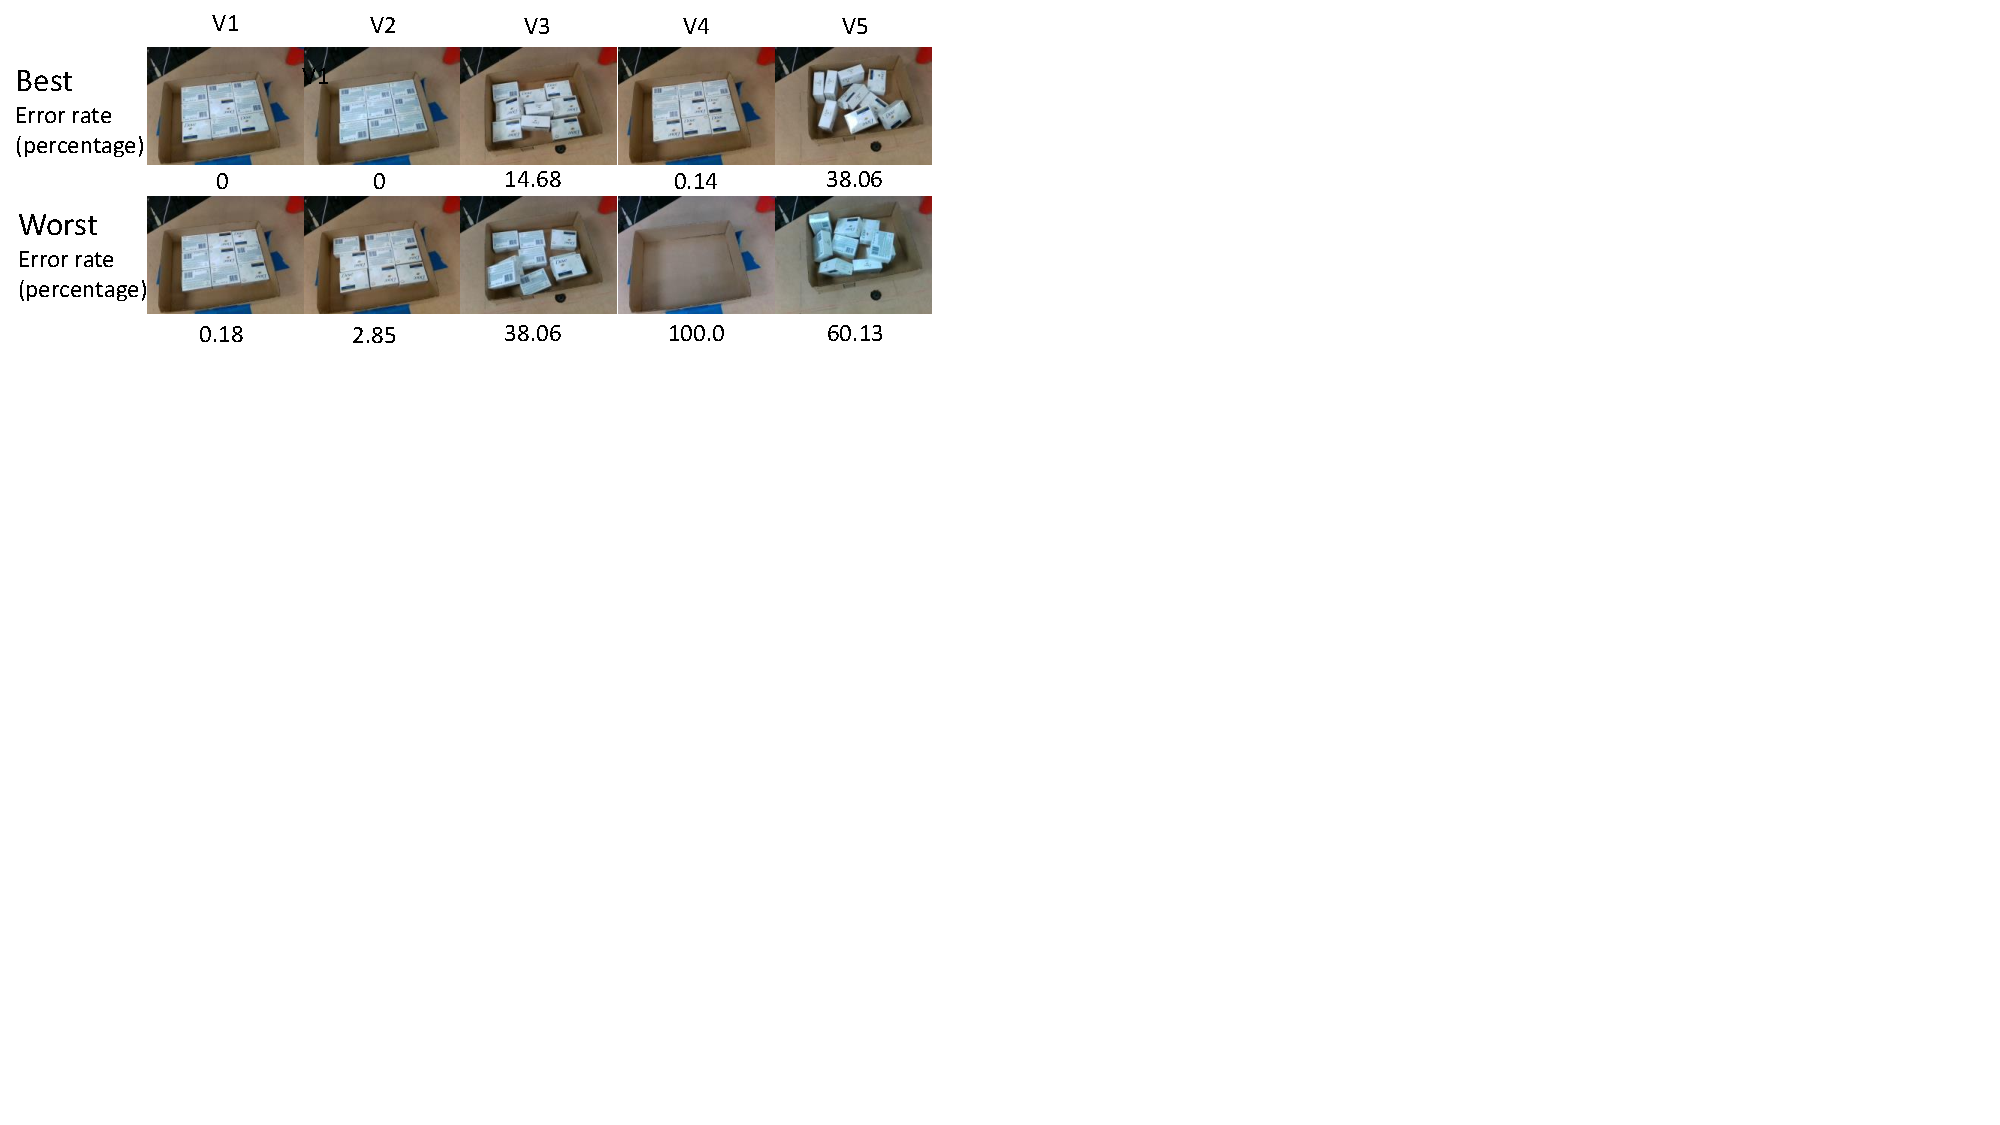
\includegraphics[width=0.9\textwidth]{Figures/final_packing.pdf}
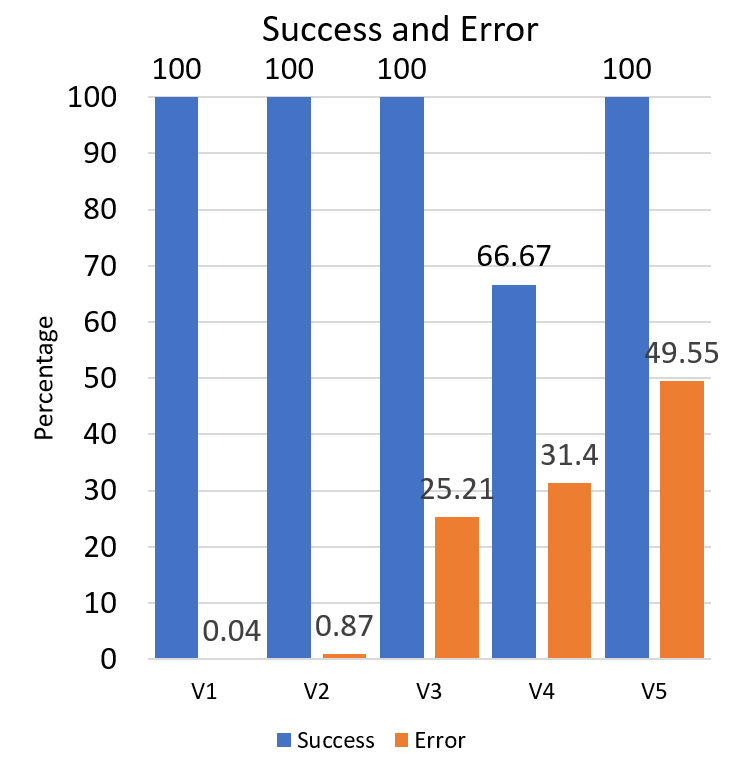
\includegraphics[height=2in]{Figures/histogram.png}
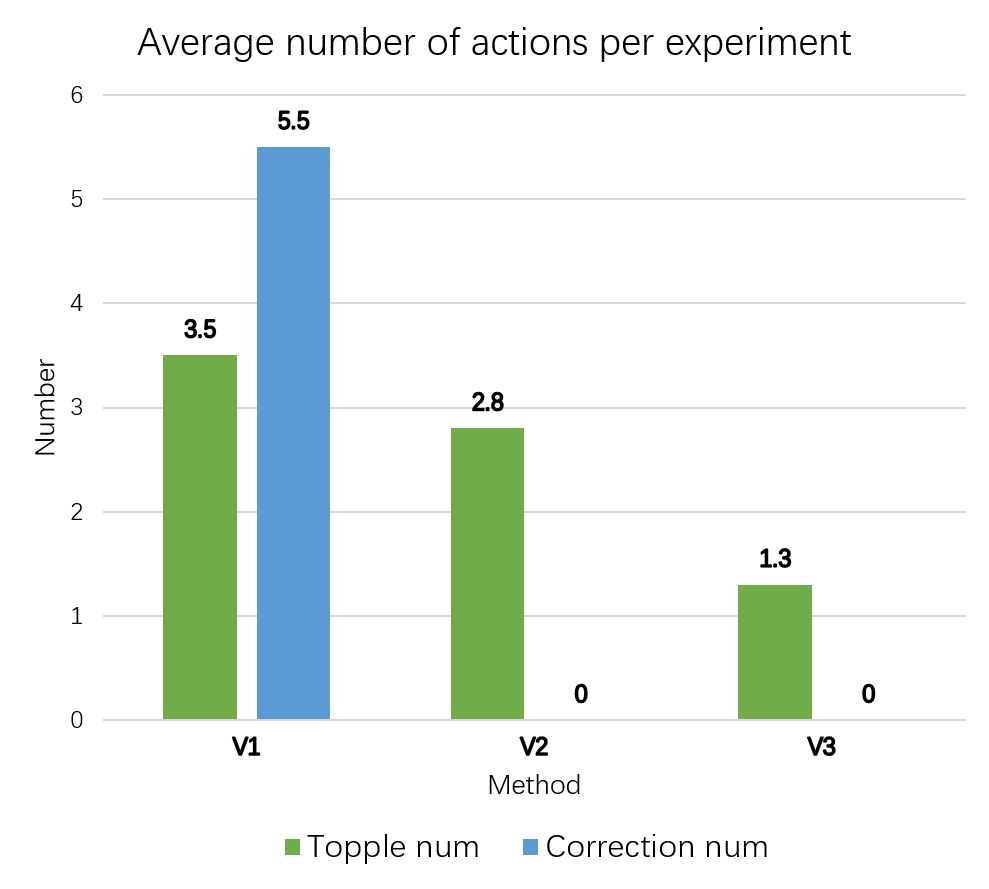
\includegraphics[height=2in]{Figures/action_num.png}
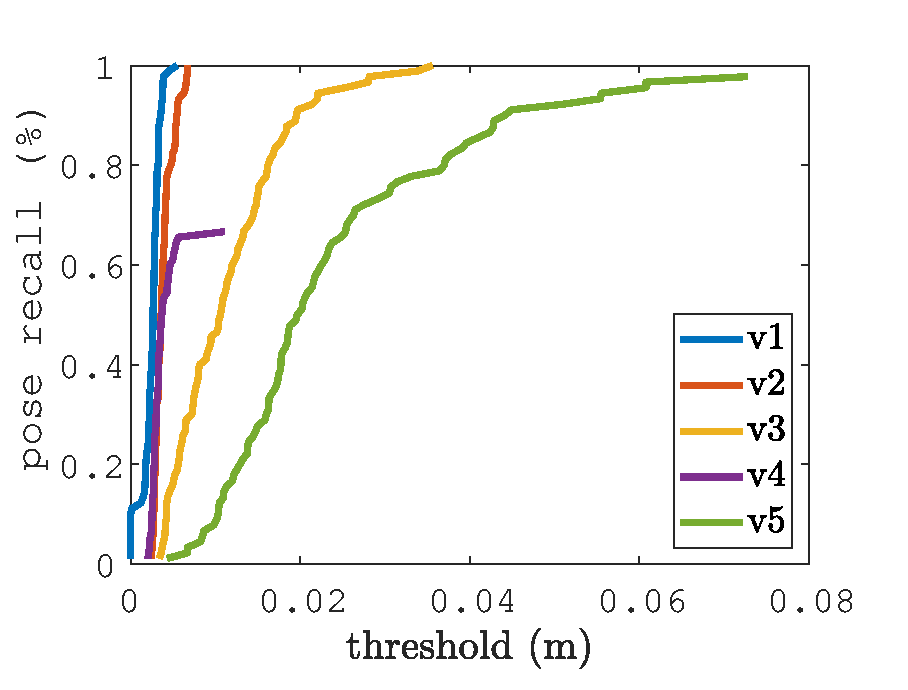
\includegraphics[height=2in]{Figures/real.eps}
\vspace{-0.1in}
\caption{(\textit{Left}): the blue bar represents the fraction of successful object transfers, the orange bar represents the percentage of unoccupied volume within the ideal target placement volume.(\textit{Middle:})\commentadd{the blue bar represents the average number of correction actions happened per experiment, the green bar represents the average number of toppling actions happened per experiment.}  (\textit{Right:}) The pose recall percentage over different thresholds is shown for the pipeline versions.
}
% \vspace{-0.2in}
\label{fig:real_data}
\end{figure*}

For consistency, an identical version of the problem is tested, with ``dove soap bars'' that are randomly thrown into the source bin $\binit$, which is placed on one side of the robot's reachable workspace (Fig \ref{fig:new_setup}). Only top-down grasps are allowed within a given alignment threshold. The start arrangement $\ainit$ of objects is intended to reflect a random pile, with $10$ repetitions of each experimental condition. The target bin $\btarget$ contains a $3\times 3$ grid arrangement of $9$ objects, on the same plane, with the stable face of the object targeted for placement. The complete pipeline uses a) corrective actions for fine adjustments, b) push-to-place actions for robust placement, c) toppling actions for increasing successes, and d) pose estimation for adjusting the object. The improvements introduced by these strategies are evaluated through the following comparison points, within the context of the proposed pipeline: 

\noindent \textbf{V1 - \commentadd{Full pipeline}}: The complete pipeline with all the primitives achieves the highest accuracy and success rate.

\noindent \textbf{V2 - No corrective actions}: The experiment corresponds to the use of \textbf{V1} without the fine correction module of Fig. \ref{fig:finer_fix}.

\noindent \textbf{V3 - No push-to-place actions}: This version is \textbf{V2} without the use of the robust placement module (Fig. \ref{fig:adaptive-pushing}) that performs push actions to achieve robust placement.

\noindent  \textbf{V4 - No toppling actions}: These experiments used \textbf{V2} without considering toppling actions to deal with objects not exposing a valid top surface that allows the target placement. 

\noindent  \textbf{V5 - (Baseline) No push-to-place, toppling, pose-estimation}: The naive baseline that solely uses a pose-unaware grasping module that reports locally graspable points and drops the grasped object at an end-effector pose raised from the center of the desired object position, with no adjustment in orientation. 

The metrics evaluated include the fraction of successful object transfers that succeed in moving objects to the target bin. The accuracy is captured in the threshold mentioned in Eq.~\eqref{eq:satisfaction} that is expressed in terms of a percentage of unoccupied volume within the ideal target placement volume. This was measured with a voxel discretization sufficient to elucidate the difference between the methods. The average data recorded is reported in Fig.~\ref{fig:final_bin_configs}. This error measure is proportional to the accuracy. The points to note for every version are detailed as follows.

%\begin{table}[]
%\centering
%\begin{tabular}{rlllll}
%\multicolumn{1}{l}{}                  & \textbf{V1}               & \textbf{V2}               & \textbf{V3}                & \textbf{V4}               & \textbf{V5}                \\ \cline{2-6} 
%\multicolumn{1}{r|}{\textbf{Success}} & \multicolumn{1}{l|}{1}    & \multicolumn{1}{l|}{1}    & \multicolumn{1}{l|}{1}     & \multicolumn{1}{l|}{0.67} & \multicolumn{1}{l|}{1}     \\ \cline{2-6} 
%\multicolumn{1}{r|}{\textbf{Error}}   & \multicolumn{1}{l|}{0.04} & \multicolumn{1}{l|}{0.87} & \multicolumn{1}{l|}{25.21} & \multicolumn{1}{l|}{31.40}    & \multicolumn{1}{l|}{49.55} \\ \cline{2-6} 
%\end{tabular}
%\label{table:success_accuracy}
%\caption{The successful object transfers and the error measure over $10$ runs of the different versions of the pipeline, packing $9$ objects per experiment.}
%\end{table}



The low error for \textbf{V1} corroborates the final bin placement evidence. On average $7$  corrective actions per experiment were invoked to achieve the high degree of accuracy.

The accuracy improvement obtained from corrective actions is evaluated in \textbf{V2}. While this version succeeded in dropping all the objects close to the correct target poses, application use-cases where a higher degree of accuracy is desired motivate the use of corrective actions. The integration of the corrective actions was done with higher error threshold during intermediate steps, and a much finer one for the final adjustment. Errors can typically arise from execution failure and pose misalignments. The less accurate these underlying processes are, the more important corrective actions become. 

\textbf{V3} only performs adjustments using pose estimation, and toppling. While, this is sufficient to successfully transfer all the objects, any difference of accuracy to \textbf{V2} would be introduced by the lack of push-to-place actions. Here there is complete reliance on the exactness of the execution and pose adjustments. Due to the proximity of adjacent object surfaces in the target grid arrangement, even minor errors get aggravated. However, due to the ability to reason about toppling, all the objects can be transferred to the target bin, even with this low accuracy. This is demonstrated in the occurrence of the failure to transfer all the objects. 

In \textbf{V4} any object that does not expose an permitted picking surface that makes the prehensile placement possible, is not picked. Any instance of the source bin, which ends with no such objects results in no valid picking actions that can make the approach proceed, and a failure is declared. The current behavior of \textbf{V4} drops the object if it is mistakenly grasped from the wrong surface. This can itself be used as a naive toppling primitive. It is important to note that there might be other alternative strategies that can deal with this failure, but the intent of this comparison is to demonstrate the importance of having a deliberate toppling strategy in the pipeline, that can change the object's orientation in the context of random starting arrangements of the object.  On average, over \textbf{V1, V2,} and \textbf{V3} the toppling primitive was required $4$ times per experiment. This highlights the necessity of this reasoning. Deliberate toppling however requires at least one additional pick action. The number of pick attempts per successful object transfer was $2.56$ for \textbf{V4}, whereas, in \textbf{V2} the same was $1.98$. This indicates that toppling is indeed necessary both in terms of success and efficiency of actions.  

Expectedly, \textbf{V5} has the lowest accuracy. However, since there is no reasoning about the pick surface, every object was transfered to the space of the bin. This has no guarantee to work if the object is larger. This drives the motivation for using a set of robust primitives for the packing problem.

Overall, the time for the experiments show a trend of increasing with the increasing complexity of the pipeline. The trade-off of accuracy versus time persists. On average, \textbf{V1} ran for $945$s while \textbf{V5} ran for $323$s.

% \begin{wrapfigure}[13]{r}{1in}
% \vspace*{-6mm}
%   \begin{center}
%   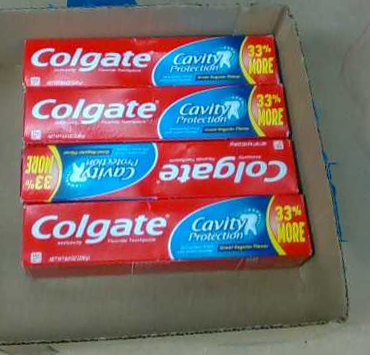
\includegraphics[width=1in,height=0.8in]{Figures/toothpaste.png}
% %  \smallskip\par
% \vspace{0.001in}
%   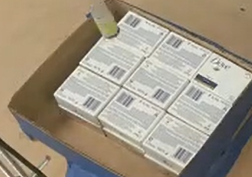
\includegraphics[width=1in, height=0.8in]{Figures/two_layer.PNG}
%   \end{center}
% \vspace*{-4mm}
%   \caption{Result for toothpaste and two-layer packing}
% \end{wrapfigure}


\subsection{Real-world Demonstrations}

Various demonstrative packing tasks (Fig~\ref{fig:final_bin_configs} \textit{bottom}) were executed to showcase the versatility of the proposed pipeline.

\noindent\textbf{Multi-layer packing}: With a sufficiently tall bin, objects can be packed in multiple layers. Running the method beyond the first plane of the grid effectively shifts all the operations to the higher plane. This is demonstrated in a standalone run.

\noindent\textbf{Different objects}: To validate the applicability of the method to other cuboidal objects, \textbf{V1} was performed for toothpastes. Over $5$ experiments,  with $4$ objects, every run succeeded in placing the object inside the bin.

\noindent\textbf{Heterogenous pile}: The source bin was filled up with two different kinds of objects and the pipeline was executed for each object sequentially, i.e., pack the \textit{toothpaste} first, and then the \textit{soap}, into two separate containers. The method is correctly capable of retrieving, and packing the desired objects from such a heterogeneous pile.

\noindent\textbf{Narrow-face reorientation}: The packing orientation is tested with the narrow (unstable) face of the cuboid being the contact surface. In such situations toppling has to reorient the object from its more stable wider face to the desired narrow face. 

\noindent\textbf{No-clearance Packing}: The target bin is resized to be of the exact dimensions as the cross section of the target arrangement. This leaves no clearance for the object for placements along the edges and corners of the $3\times 3$ grid. The compliance of the end-effector, and walls of the container are leveraged in the extended variant of the adaptive pushing primitive, to allow successful application of the proposed pipeline in this setting.

\rahul{


\subsection{Simulation: Adaptive Pushing}

\begin{figure*}[ht]
    \centering
    \begin{overpic}[height=1.4in]{Figures/vol_err_plot.png}%
    \put(450,-50){(a)}%
    \end{overpic}
    % 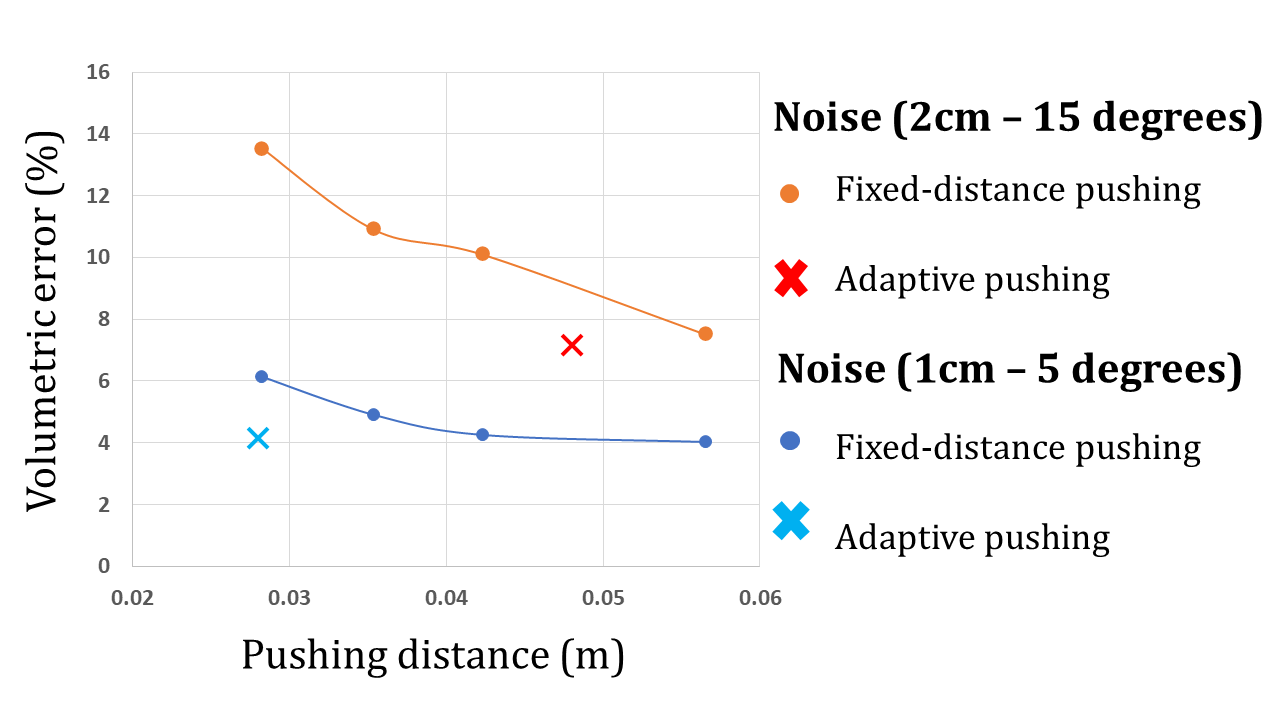
\includegraphics[height=1.4in]{Figures/vol_err_plot.png}
    \begin{overpic}[height=1.55in]{Figures/expansion_higher_noise.eps}%
    \put(450,-50){(b)}%
    \end{overpic}
    % 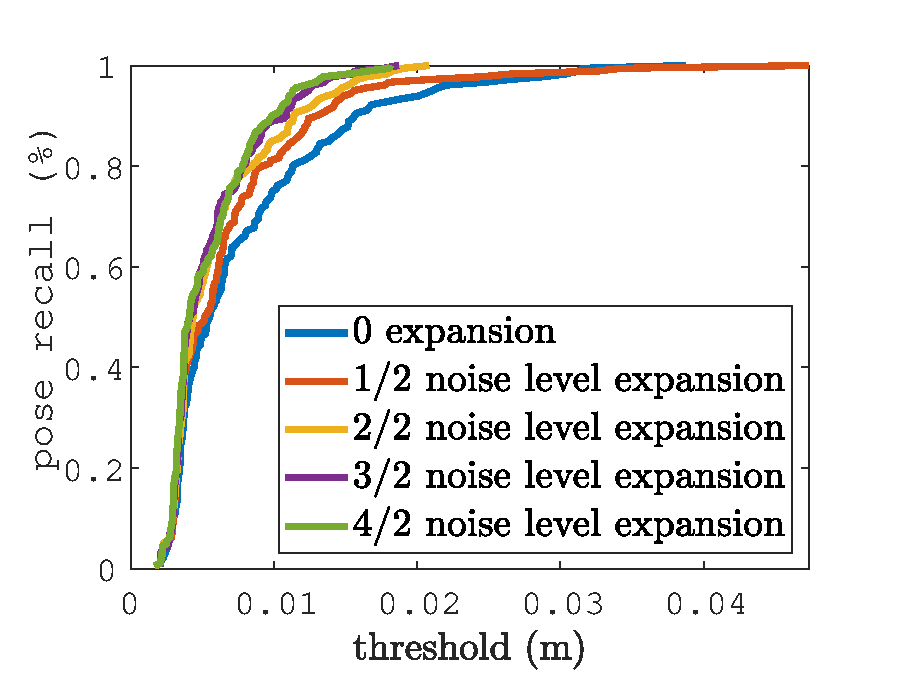
\includegraphics[height=1.55in]{Figures/expansion_higher_noise.eps}
    \begin{overpic}[height=1.55in]{Figures/z_lift_higher_noise.eps}%
    \put(450,-50){(c)}%
    \end{overpic}   
    % 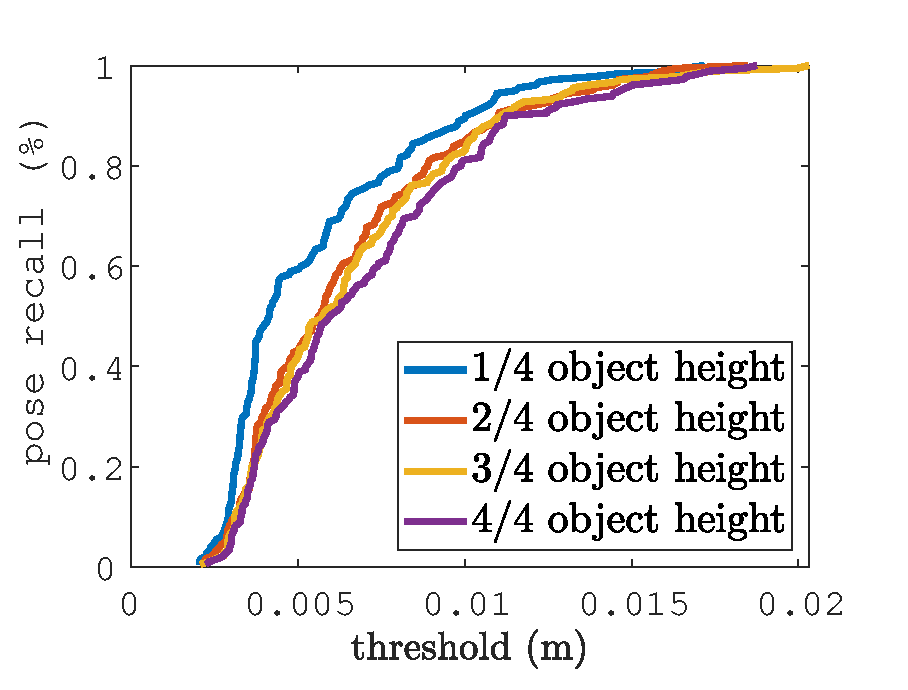
\includegraphics[height=1.55in]{Figures/z_lift_higher_noise.eps}
    \caption{(\textit{a}) Volumetric error of proposed adaptive pushing primitive compared with baseline method under two noise levels. Pushing distance is a parameter for the baseline method. 
    Pose recall against the parameter for adaptive pushing. \textit{b} expansion size of object model, \textit{(c)} height of pre-push pose
    }
    \label{fig:adaptive-pushing-compare}
\end{figure*}

To examine the effectiveness of proposed adaptive pushing primitive on reducing the packing error, experiments were executed to compare proposed method with a simple baseline method. For each new object to place, given the target pose, the baseline method will calculate a pre-push pose using a fixed displacement. During the simulation, uniform random noise is applied to the pre-push pose in both translation and rotation direction, to evaluate the performance under different level of noise, two noise levels are introduced. The lower noise level applies 1 cm deviation to the translation direction and 5 degrees deviation to the rotation direction, while the higher noise level applies 2 cm deviation and 15 degrees accordingly. 
In the experiment, the proposed method is compared against the baseline method with different fixed displacement as parameters. The result is shown in Fig \ref{fig:adaptive-pushing-compare}. From the result, we can observe that as the pushing distance decreases for the baseline method, its performance becomes worse compared with the proposed adaptive primitive. When the pushing distance is larger than 5cm, the baseline method's performance is better than the adaptive primitive, but large fixed pushing distance will also cause issues in restricted space such as in the packing scenario. 
% \begin{figure}
%     \centering
%     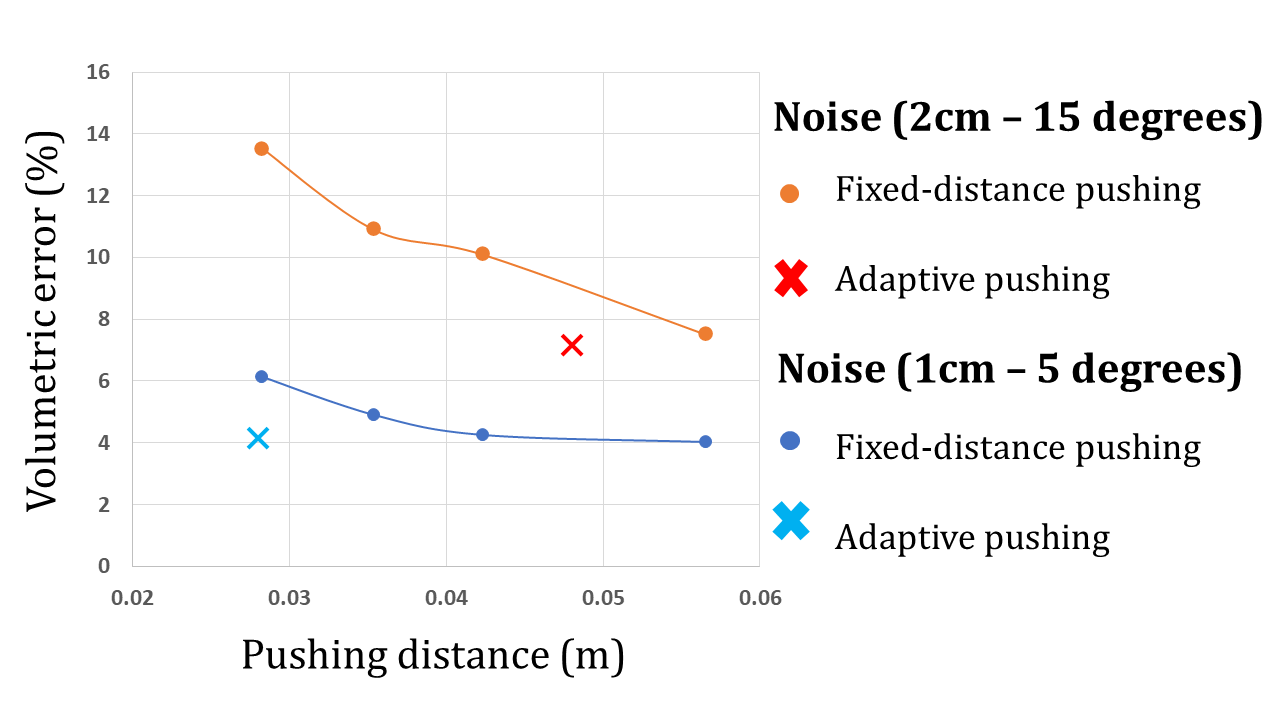
\includegraphics[width=0.5\textwidth]{Figures/vol_err_plot.png}
%     \caption{Volumetric error of proposed adaptive pushing primitive compared with baseline method under two noise levels. Pushing distance is a parameter for the baseline method. }
%     \label{fig:adaptive-pushing-compare}
% \end{figure}

% \begin{figure}
%     \centering
%     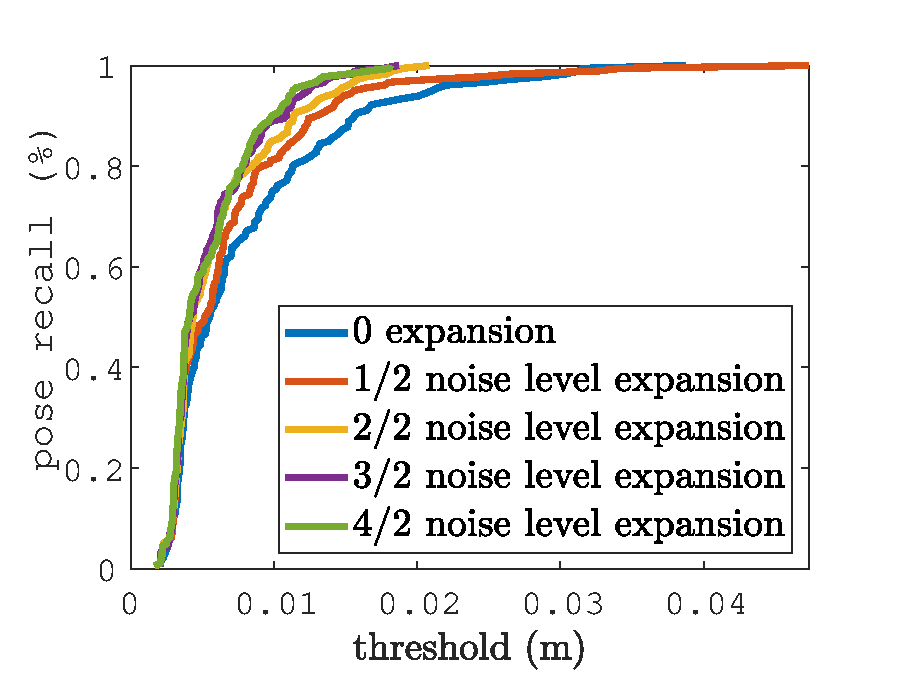
\includegraphics[width=0.49\linewidth]{Figures/expansion_higher_noise.eps}
%     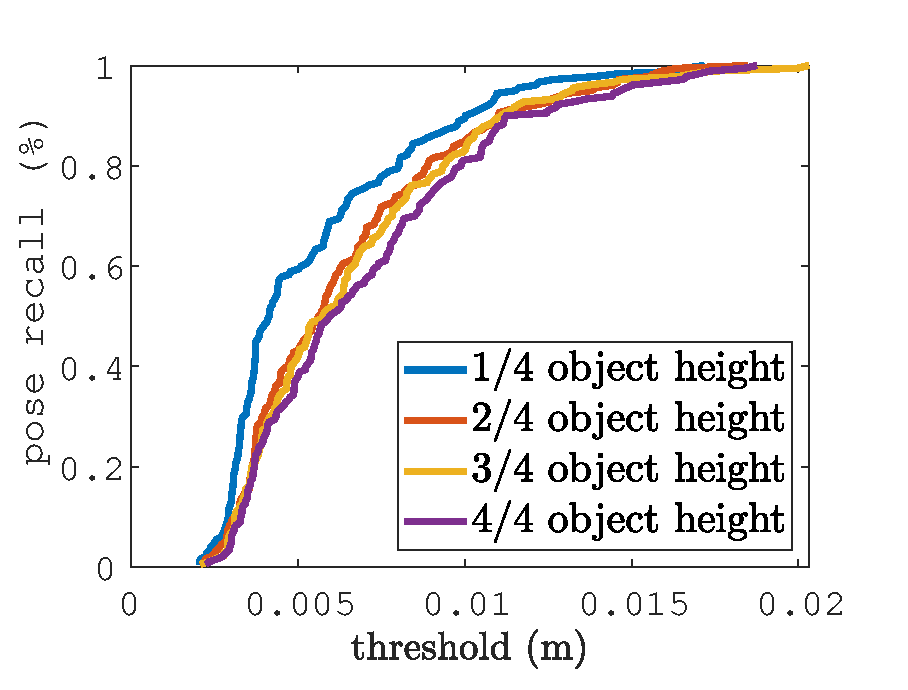
\includegraphics[width=0.49\linewidth]{Figures/z_lift_higher_noise.eps}
%     \caption{Pose recall against the parameter for adaptive pushing. (left) expansion size of object model, (right) height of pre-push pose}
%     \label{fig:expansion_simulation}
% \end{figure}




To further evaluate the adaptive pushing primitive, we have examined the influence of two parameters. The first is the expansion size of object model for collision checking, the second factor is the height of pre-push pose. The evaluation will help to determine a best strategy for choosing these parameters and also validate our understanding of proposed primitive. The result is shown in Fig \ref{fig:adaptive-pushing-compare}, two figures are corresponding to the mentioned two parameters. For the expansion size, we tested different expansions relative to the noise level and check how the pose recall changes according to the expansion sizes.  The result under higher noise is shown in the left figure, we can observe that once the expansion size drops below the noise level, the pose recall curve drops rapidly. Another observation is that the pose recall is much more sensitive to expansion size under higher noise level. Under the lower noise level, the pose recall curves are much closer to each other compared under higher noise level. At last, in order to achieve stable performance, it is best to choose expansion size that is bigger than 2 times of the noise level. 
% \begin{figure}
%     \centering
%     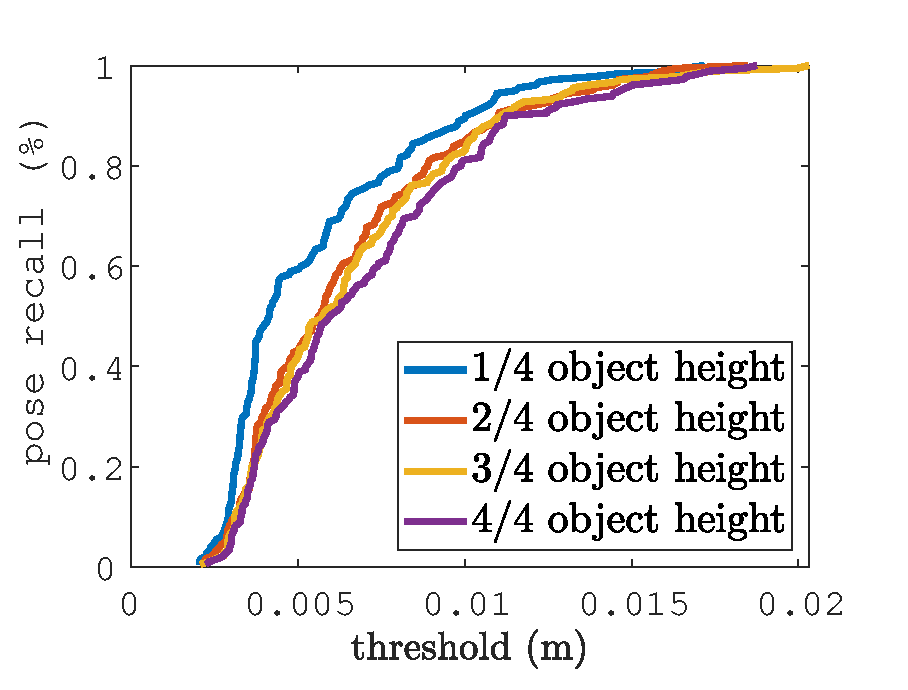
\includegraphics[width=0.49\linewidth]{Figures/z_lift_higher_noise.eps}%
%     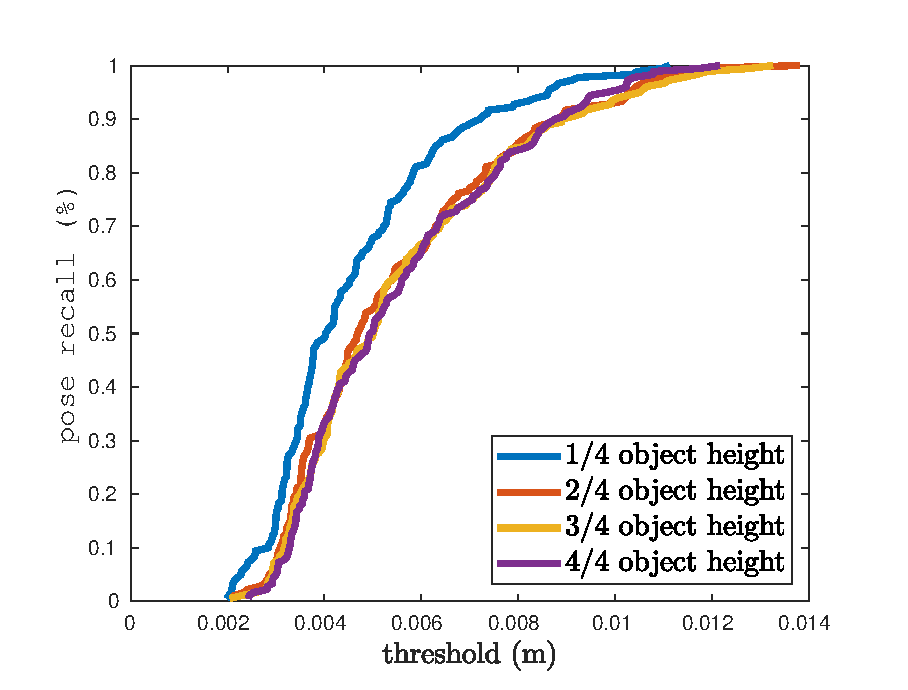
\includegraphics[width=0.49\linewidth]{Figures/z_lift_lower_noise.eps}
%     \caption{Pose recall against the height of pre-push pose}
%     \label{fig:height_pre_push_pose_simulation}
% \end{figure}
For the height of the pre-push pose, we tested different value relative to the object's height and check how the pose recall changes accordingly. The result is shown in the right figure of Fig \ref{fig:adaptive-pushing-compare}. From the figure, we can observe that the pose recall curve drops rapidly after the height of pre-push pose increases over 1/4 of object height under both noise levels. 

}

\changkyu{

\subsection{Simulation: Fine Correction}

\begin{figure*}[ht]
    \centering
    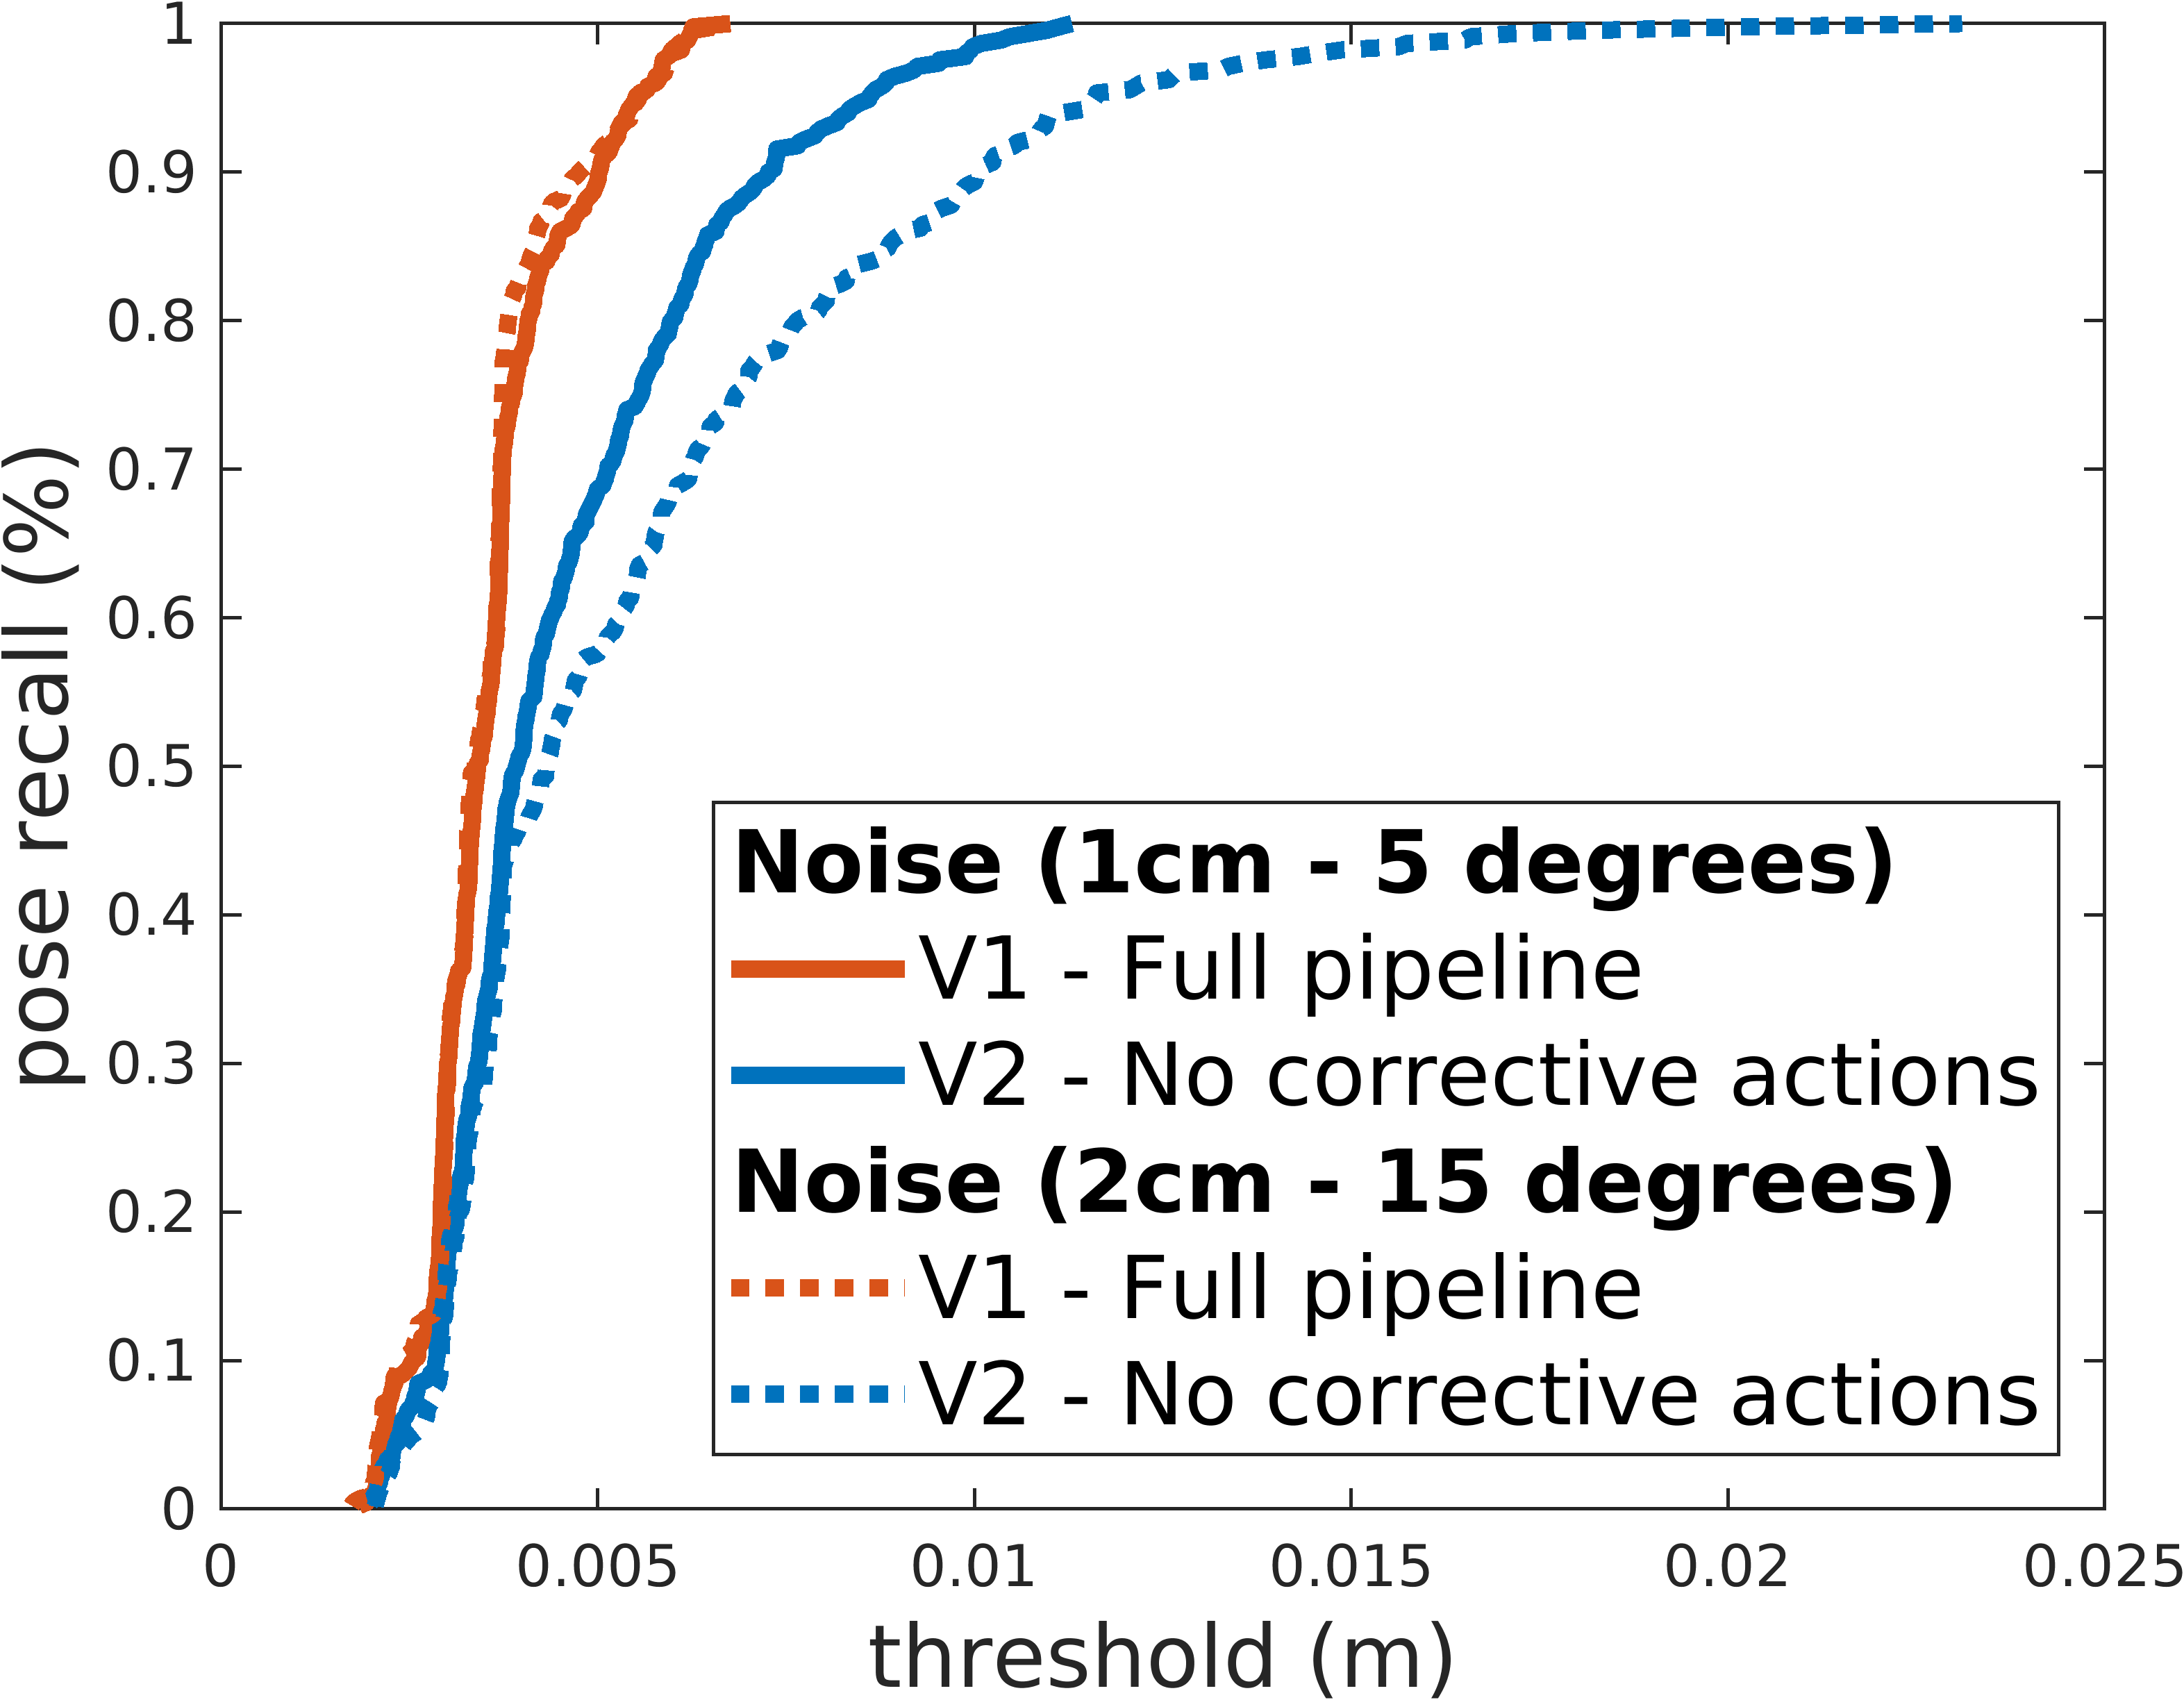
\includegraphics[width=0.34\textwidth,valign=t]{./Figures/res_recall.png}
    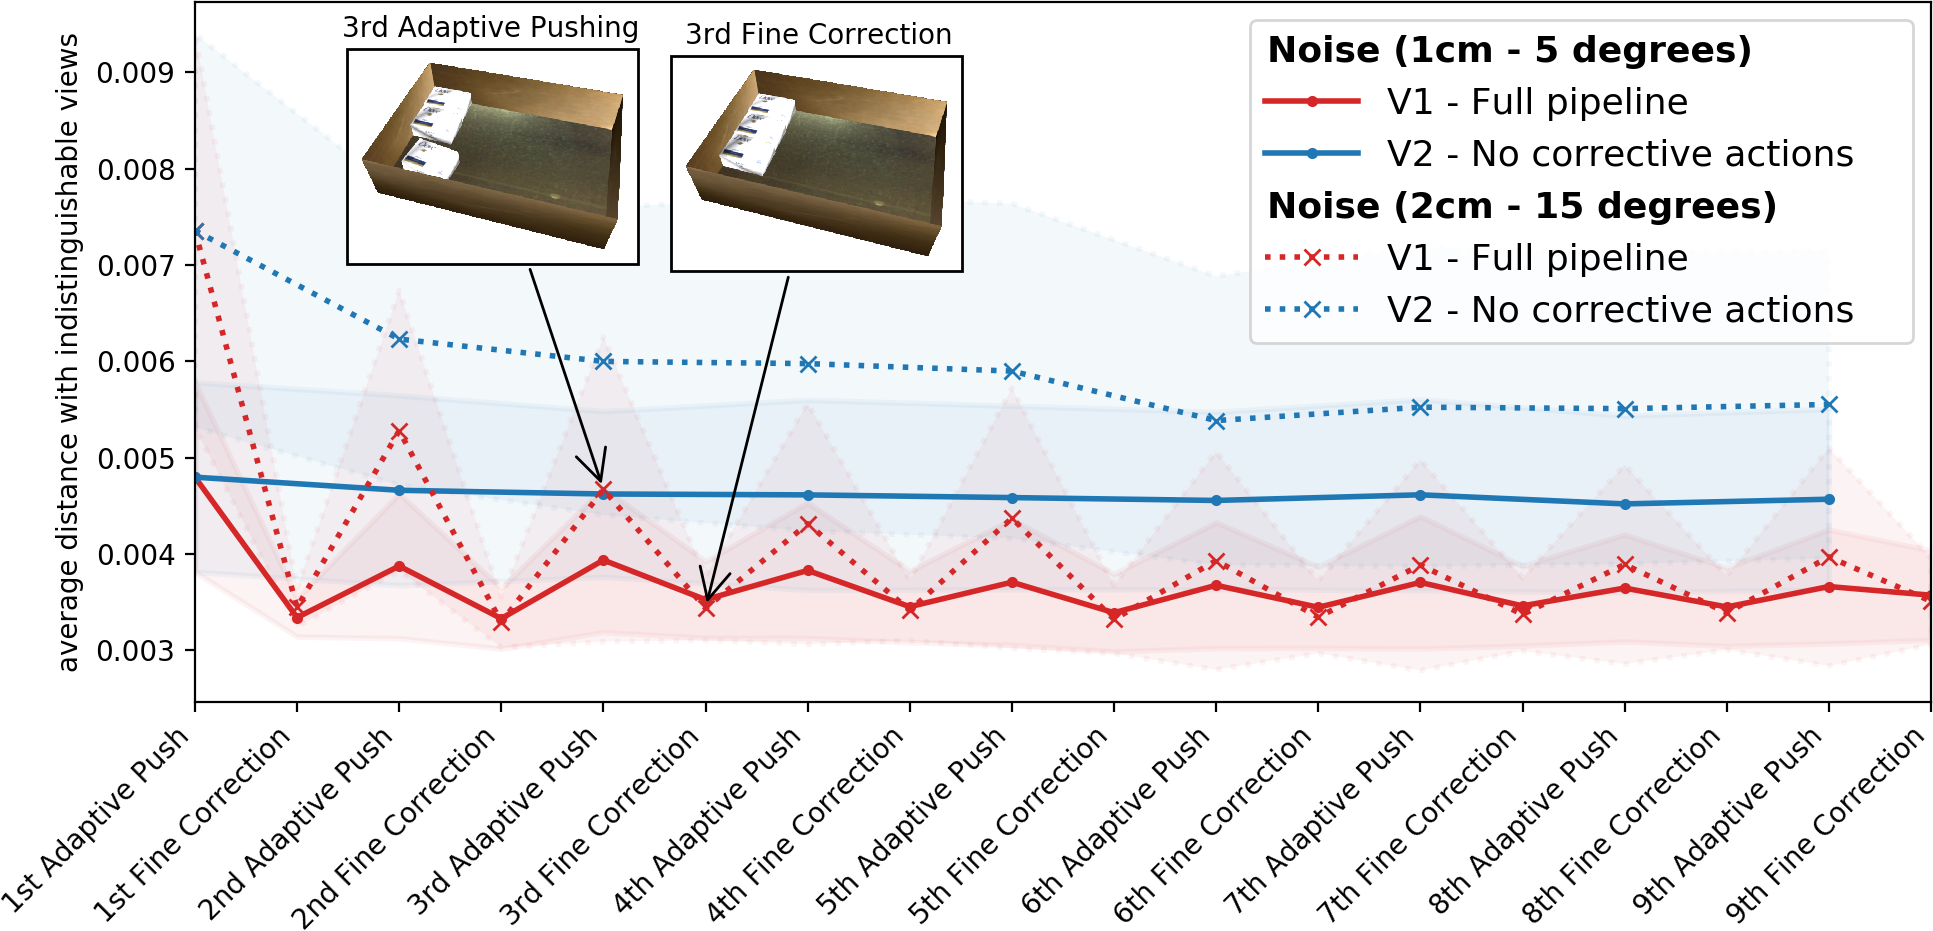
\includegraphics[width=0.64\textwidth,valign=t]{./Figures/res_step.png}
    \caption{Pose recall (left) and volumetric error (ADI) against the number of placed objects (right) with and without the fine correction module under different noise levels.}
    \label{fig:res_recall}
\end{figure*}

We evaluated the fine correction module on the same simulation setup with the same noise levels: 1cm deviation to the translation and 5 degrees deviation to the rotation, 2cm and 15 degrees deviations accordingly.
We compared \textbf{V1 - Full Pipeline} that has the all the primitives including the fine correction module and \textbf{V2 - No corrective actions} that uses \textbf{V1} but has no fine correction module.
The fine correction is repeated until the point cloud is aligned with the desired goal poses given a threshold $\epsilon=0.5cm$, but it is never repeated more than $4$ times for each placement.

Fig~\ref{fig:res_recall} (left) shows the pose recall rate under different noise levels.
In this experiment, $1.03 (\pm0.80)$ number of corrective actions are executed per placement in average.
Without the corrective module (\textbf{V2}), the pose recall curve dropped as the noise level raised.
However, the full pipeline \textbf{V1} kept a high recall rate regardless of the noises.
Fig~\ref{fig:res_recall} (right) shows the volumetric error (ADI) against the number of placed objects.
Whenever the fine correction module was executed, the volumetric error dropped under its threshold (\textbf{V1}), while the error of \textbf{V2} does not decrease dramatically.
The fine correction module not only corrected the misplacement due to the simulated noise, but also it prevents the situation that the misaligned objects affect to the future placement.

}
% Contributions of the paper we want to demonstrate and improvements relative to current version:

%  - Picking so as to expose the right surface: improve the dropping so that we reason how to reorient it but treating the original bin as a terrain

% - robust placement at the target bin: we should pick automatically the placement of the object and the direction of the pushing operation by taking into account the interaction of multiple objects (i.e., with the placement of the last object fix the orientation of the previous ones as well)

% - toppling and pushing fix: use the same reasoning about the interaction of multiple objects 

% Comparison Experiment, One 3x3 layer (without foam):

% A. Base case - without pose estimation, find a flat surface in the source and drop it in a pre-defined location (drop from higher distance)
 
% B. With pose estimation, prioritizing flat surface, trust the original pose estimation, you go directly at the target configuration but drop from a height

% C. Same as before but verifying at the source bin: with dropping the object when we detect that we picked the wrong surface

% D. Same as before but verifying at the target bin: pushing operation - first time we place at the bottom of the bin

% E. Same as before but we also evaluate success from vision and perform toppling and pushing operations directly from data so as to maintain an invariant of packed objects

% Demonstrations: 

%  - different object: the toothpastes
 
%  - multiple layers (without the foam)
 
%  - with the foam 

% Metrics?

%  - percent of boxes transported into the target bin
 
%  - distance from preferred pose (intersection over union)
 
%  - time
 
%  - \# of grasps, \# of times we topple (and how many times we succeeded), \# of times we fix the placement of objects (and how many times we succeeded) 

% Save the videos for all the experiments in a URL

% Bring up in the discussion section of the paper the following future work points: 

%  - what if the side you need to pick it up is the unstable one?
 
%  - perform the robust placement in SE(2) instead of R(2)

% - topple directly objects if there is no good surface exposed

% - the location of the bin may not be known

% - we want to eventually place object of different types in 
%  the same bin